\documentclass{article}
\usepackage[french]{babel}
\usepackage[T1]{fontenc}
\usepackage[utf8]{inputenc}
\usepackage{graphicx}
\usepackage{eurosym}
\usepackage {times}
\usepackage{fancyhdr}
\usepackage{bm}
\usepackage{listing}
\title{Projet CamlT'OCR par SMK \~Cahier des charges}
\pagestyle{fancyplain} \lhead{\textit{Projet DotNet}} \rhead{\textit{KMnO4}}
\date{24-10-2014}
\author{
    Timothe \textit{Tim-Tim} Bureau-Godart(bureau\_t) \and
        Leopold \textit{Meta} Szabatura (szabat\_l) \and
        Louis \textit{Zab} Forget (forget\_l) \and
        Maxime \textit{Kylox} Gaudron (gaudro\_m)
        1      }


\begin{document}
\begin{center}
\maketitle
\end{center}
\newpage
\tableofcontents
\newpage
\section{Introduction}
\addcontentsline{toc}{section}{Introduction}
Dans le cadre de notre specialisation en informatique a l'EPITA, nous avons eu comme projet smestrielle la realisation d'un ocr ( Optical Character Recognition). Ce projet ce deroule sur 4 mois en Ocaml, un langage develloper par l'INRIA. Nous presentons donc dans ce rapport l'etat d'avancement du projet a la vielle de la premiere soutenance. Ce projet a ete realise par quattre membre fidele et devoue a la bonne cause celle de notre ocr ! 
\subsection{presentation des membres}
\subsubsection{Louis "\textit{Zab}" Forget}
J'ai toujours etais tres curieux, au point de partir souvent dans tous les sens. J'ai toujours voulu savoir comment marchent les pages webs. C'est dans cette optique que j'ai appris a faire du HTML et CSS en troisieme. J'ai ensuite voulu savoir comment marchent les jeux videos, puis divers programmes. Il y a quelques jours je me suis demandais commemt marchent les gps qui indiquent la densite du traffic.
\subsubsection{Timothe "\textit{Tim-Tim}" Bureau Godart}
\subsubsection{Leopold "\textit{Meta}" Szabatura}
\subsubsection{Maxime "\textit{kylox}" Gaudron}
J'ai toujours vecu dans un monde plus ou moin informatiser. Adepte de tout les petits appareil electronique et mecanique. A tel point que je demontais tout et que plus rien ne marchait ! Je me suis donc mis naturellement a aller chercher un peu plus loin dans le fonctionnent interne des appareils. L'ocr est donc pour moi un grand apprentissage et une decouverte qui permet d'envisager differente possibilite de reconnaissane et de systemes automatiser ! 
\subsection{organisation du projet}
\newpage
\section{Les taches}
\subsection{quelque mots sur le site internet}
\subsection{Interface graphique}
\subsection{Traitement d'image}
\subsubsection{Le niveau de gris}
\subsubsubsection{\textbf{Le concept}}:\\
Une image se compose d'element appeler pixel et definie par trois composante (en realite quattres mais ceci est une autre histoire) qui sont R,G et B correspondant au valeur Red, Green et Blue d'un pixel. Cette etape est primordiale car elle va permettre le bon traitement de l'image par l'ensemble des etapes aui la succede.\\
\subsubsubsection{\textbf{La realisation}}:\\
Pour realiser ce niveau de gris on va travailler sur le trois composante d'un pixel et appliquer la fromule suivante :
\\
\begin{center}
\[x = \frac{0.299 \times R + 0.587 \times G + 0.114 \times B}{3}\]
\end{center}
a l'ensemble des pixels de l'image. Le niveau de gris est operationel dans notre ocr, nous pouvons donc passer a la tache suivante.
\begin{figure}[h]
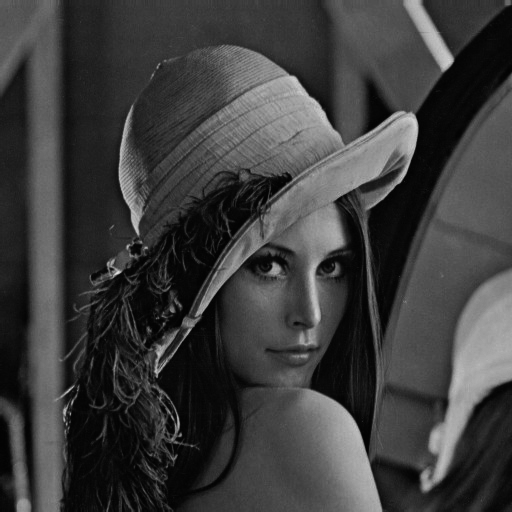
\includegraphics[width=0.50\textwidth]{img/grey.png}
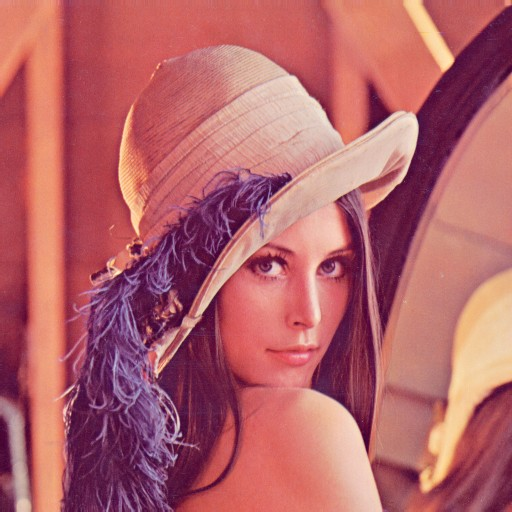
\includegraphics[width=0.50\textwidth]{img/lena.jpg}
\caption{avec et sans nuance (captain obvious is obvious)}
\end{figure}
\newpage{}
\subsubsection{Le filtre median}
\subsubsubsection{\textbf{Le concept}}:\\
Le filtre median va pour chaque pixels de l'image recupere le triplet (R,G,B) de chaque pixel autour du pixel traite et trier ces pixels par ordre croissant. Il suffit juste de recuperer la valeur mediane de la liste trier. Le passe dans cette algo et qyue l'on doit passer les pixels sur une autre image pour pas fausser les calculs sur la premiere image !
\subsubsubsection{\textbf{La realisation}}\\
En pratique ce filtre ne s'applique pas sur toute les images car sinon elle floute l'image et la rend intraitable. Je suis actuellement en recherche d'un algorithme permettant de palier ce gros probleme. Au niveau aulgoritemiaue on obtiens
\begin{figure}[h]
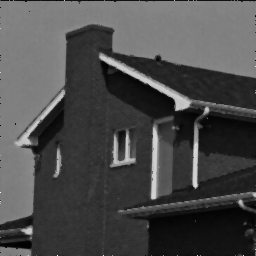
\includegraphics[width=0.50\textwidth]{img/house.png}
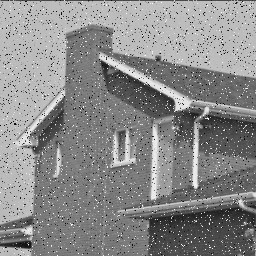
\includegraphics[width=0.50\textwidth]{img/house.jpg}
\caption{presentation du filtre median}
\end{figure}
\subsubsection{La binarisation}
\subsubsubsection{\textbef{Le concept}}:\\
Nous utilisons l'algorithme d'Otsu, du nom de son inventeur Nobuyuki Otsu. Qui se base sur l'histogramme d'un image. L'histogramme est un tableau de 255 element, ici des entiers, qui represente le nombre d'occurence d'un niveau de gris ( les niveau de gris allant de 0 (blanc) a 255 (noir). Dans un permier temps va creer un tableau pour y mettre les valeur traiter de l'histogramme de la maniere suivant 
\begin{center}
\[ p_{i} = \frac{h_{i}} {width * height}\]
\end{center}
qui renvoie la population du niveau de gris i dans l'ensemble des pixels de l'image.
\subsubsection{rotation}
Je me suis donc occupe de la transformation de Hough. La transforme de hough est une techmiaue de reconnaissance de formes invente en 1962 par Paul Hough.
Le principe qui sous-tend la transforme de Hough est qu'il existe un nombre infini de ligne passant par un point dont la seule difference est l'orientation (l'angle). La transforme generalise de Houg fonctionne sur le principe qu'une droite peux s'ecrire sous la forme 
\[r = x\cos{\theta}+y\sin{\theta}\]
A chaque pixels noir on essaye de trouver la vlauer maximum de r. Cette valeur represente la droite qui alligne le plus de pixel noir. On la retiens et on vote dans un tableau pour son angle associer. On recommence sur tout les pixels. L'angle qui a recu le plus de vote estl'anlge de rotation de l'image( minore de la moitier de l'intervalle pour pouvoir faire ressortir les angles negatifs). 
\begin{figure}[hp]
\centering
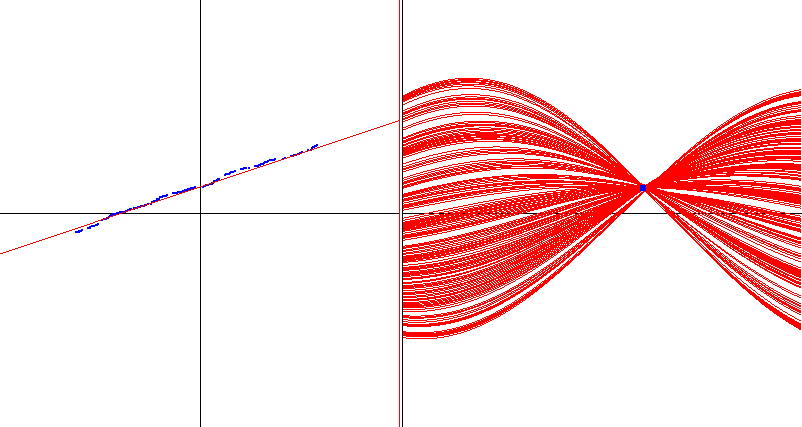
\includegraphics[width=0.80\textwidth]{img/hough.png}
\end{figure}
\subsection{Decoupage de l'image}
\subsection{Perceptron}
\section{Conclusion}


\end{document}
